\documentclass{article}
\usepackage[utf8]{inputenc}
\usepackage[a4paper, total={6.5in, 9.5in}]{geometry}
\usepackage{float}
\usepackage{amsmath}
\usepackage{amssymb}
\usepackage{mathtools}
\usepackage{tensor}
\newcommand{\torseur}[7]{
\tensor[_{#1}]{\left\{ \begin{array}{cc}
    #2 & #5 \
    #3 & #6 \
    #4 & #7
\end{array} \right\}}{_{(\vec{x};\vec{y};\vec{z})}}
}
\usepackage{siunitx}
\sisetup{output-decimal-marker={,},group-minimum-digits=4,abbreviations}
\sisetup{inter-unit-product=\ensuremath{{}\cdot{}}}
\newcommand{\deftable}[2]{%
%\hline
\textbf{B.A.M.E}
\begin{table}[h]
    \centering
    \begin{tabular}{llp{130mm}}%
        %& unité/type & Explication \ \hline
        #1
    \end{tabular}
    \label{tab:#2_units}
\end{table}%
}
\newcommand{\deftablevar}[3]{%
    $#1$ & $\si{#2}$ & #3 \
}
\newcommand{\deftableobj}[3]{%
    $#1$ & \textit{#2} & #3 \
}
\newcommand{\bame}[1]{%
%\hline
\begin{table}[h]
    \centering
    \begin{tabular}{llllp{130mm}}%
        Nom & Vecteur & Direction & Sens & Norme \hline
        #1
    \end{tabular}
\end{table}%
}
\newcommand{\vect}[1]{\overrightarrow{#1}}

\title{Suspension VTT}
\author{Ewen Le Bihan}
\date{2020-05-28}

\begin{document}

\maketitle

\section{}

\begin{align*}
	\sigma&= \frac{N}{a^2\cdot 2} \\
	      &= \frac{10 000}{2\cdot a^2}
.\end{align*}

\section{}

\begin{align*}
	\sigma&= \frac{10000}{2\cdot 8^2} \\
	      &= \frac{10000}{128} \\
	      &= \SI{78.125}{\mega\pascal}
.\end{align*}


\section{}

La limite d'élasticité de l'alliage d'aluminium 7075 est de $\SI{440}{\mega\pascal}$, or $78.125 < 440$, donc la pièce est assez résistante

\section{}

\begin{figure}[h]
	\centering
	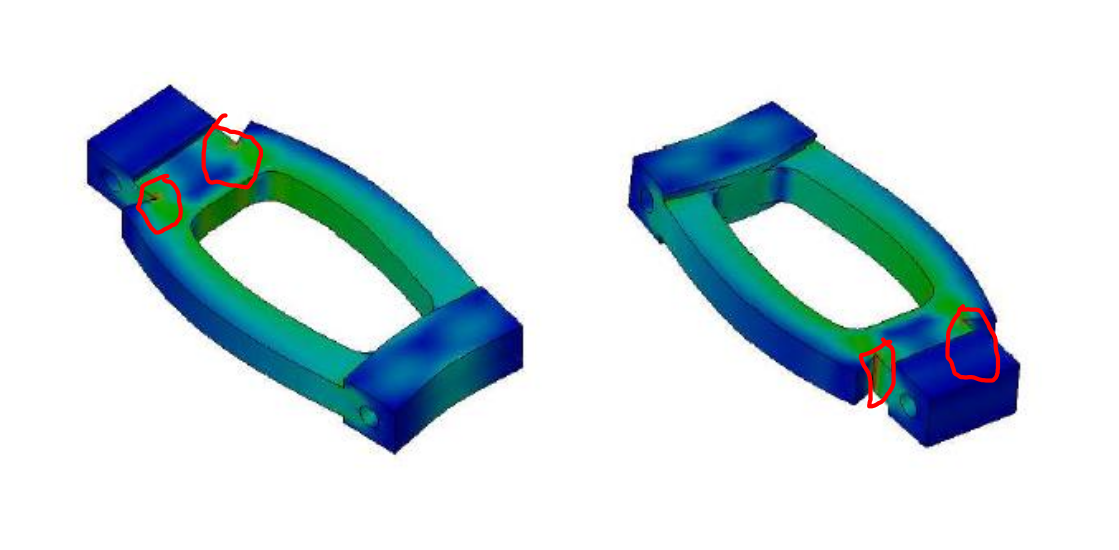
\includegraphics[width=0.8\textwidth]{points-de-fortes-contraintes.png}
	\caption{Points de fortes contraintes}
	\label{fig:points-de-fortes-contraintes}
\end{figure}

\section{}
La contrainte maximale est de $\sigma_{\text{max}} = \SI{28.7E8}{\pascal} \quad\text{soit}\quad \SI{287}{\mega\pascal}$. $287 < 440$, donc la pièce ne se cassera pas.

\end{document}
